\documentclass[12pt]{article}
\usepackage[a4paper, margin=0.75in]{geometry}
\usepackage[document]{ragged2e}
\usepackage{graphicx}
\graphicspath{ {./images/} }
\usepackage{enumerate}
\usepackage{framed}
\usepackage{amsmath,amsfonts,amsthm,thmtools,amssymb,mathtools,commath}
\usepackage{physics}
\usepackage{tikz}
\usetikzlibrary{mindmap}
\usepackage{caption}
\usepackage{xcolor}
\usepackage[most]{tcolorbox}
\usepackage{cleveref}


%%%%%%%%%%%%%%%%
%  Definition  %
%%%%%%%%%%%%%%%%
\tcbuselibrary{theorems,skins,hooks}
\newtcbtheorem[number within=subsection]{definition}{Definition}%
{
    % theorem style=definition,
    enhanced,
	before skip=2mm,after skip=2mm, colback=cyan!5,colframe=cyan!80!black,boxrule=0.5mm,
	attach boxed title to top left={xshift=1cm,yshift*=1mm-\tcboxedtitleheight},
	boxed title style={frame code={
					\path[fill=cyan]
					([yshift=-1mm,xshift=-1mm]frame.north west)
					arc[start angle=0,end angle=180,radius=1mm]
					([yshift=-1mm,xshift=1mm]frame.north east)
					arc[start angle=180,end angle=0,radius=1mm];
					\path[left color=cyan!30!black,right color=cyan!30!black,
						middle color=cyan!50!black]
					([xshift=-2mm]frame.north west) -- ([xshift=2mm]frame.north east)
					[rounded corners=1mm]-- ([xshift=1mm,yshift=-1mm]frame.north east)
					-- (frame.south east) -- (frame.south west)
					-- ([xshift=-1mm,yshift=-1mm]frame.north west)
					[sharp corners]-- cycle;
				},interior engine=empty,
		},
	fonttitle=\bfseries,
	title={#2},#1
}{def}


%%%%%%%%%%%%%
%  Theorem  %
%%%%%%%%%%%%%
\tcbuselibrary{theorems,skins,hooks}
\newtcbtheorem[use counter from=definition]{theorem}{Theorem}%
{
    theorem style=plain,
    enhanced,
    colframe=green,
    boxrule=1pt,
    titlerule=0mm,
    toptitle=1mm,
    bottomtitle=1mm,
    fonttitle=\bfseries,
    fontupper=\mdseries\itshape,
    coltitle=green!30!black,
    colbacktitle=cyan!15!white,
    colback=green!10,
    description font=\bfseries\sffamily
}{thrm}


%%%%%%%%%%%%%%
% Corollary  %
%%%%%%%%%%%%%%
 \tcbuselibrary{theorems,skins}
 \newtcbtheorem[use counter from=theorem]{corollary}{Corollary}%
 {
    theorem style=plain,
    enhanced,
    colframe=green,
    frame hidden,
    titlerule=0mm,
    toptitle=1mm,
    bottomtitle=1mm,
    fonttitle=\bfseries,
    fontupper=\mdseries\itshape,
    coltitle=green!30!black,
    colbacktitle=cyan!15!white,
    colback=green!10,
    description font=\bfseries\sffamily
 }{corl}


%%%%%%%%%%%%%
%  Example  %
%%%%%%%%%%%%%
\tcbuselibrary{theorems,skins,hooks}
\newtcbtheorem[number within=section]{example}{Example}%
{
	enhanced,
	breakable,
	colback = gray!5,
	frame hidden,
	boxrule = 0sp,
	borderline west = {2pt}{0pt}{gray},
	sharp corners,
	detach title,
	before upper = \tcbtitle\par\smallskip,
    coltitle=gray!70!black,
	fonttitle = \bfseries\sffamily,
	description font = \mdseries\bfseries
}
{xmp}


%%%%%%%%%%%%%%
%  Exercise  %
%%%%%%%%%%%%%%
\tcbuselibrary{theorems,skins,hooks}
\newtcbtheorem[number within=section]{exercise}{Exercise}%
{
    enhanced,
    breakable,
    colback=black!5,
    colframe=black!30,
    left=0.5em,
    before skip=10pt,
    after skip=10pt,
    boxrule=0pt,
    boxsep=0pt,
    arc=0pt,
    outer arc=0pt,
    borderline west={3pt}{0pt}{black!30},
}{exc}

%%%%%%%%%%
%  Note  %
%%%%%%%%%%
\usetikzlibrary{arrows,calc,shadows.blur}
\tcbuselibrary{skins}
\newtcolorbox{note}[1][]{%
	enhanced jigsaw,
	colback=gray!20!white,%
	colframe=gray!80!black,
	size=small,
	boxrule=1pt,
	title=\textbf{Note:-},
	halign title=flush center,
	coltitle=black,
	breakable,
	drop shadow=black!50!white,
	attach boxed title to top left={xshift=1cm,yshift=-\tcboxedtitleheight/2,yshifttext=-\tcboxedtitleheight/2},
	minipage boxed title=1.5cm,
	boxed title style={%
			colback=white,
			size=fbox,
			boxrule=1pt,
			boxsep=2pt,
			underlay={%
					\coordinate (dotA) at ($(interior.west) + (-0.5pt,0)$);
					\coordinate (dotB) at ($(interior.east) + (0.5pt,0)$);
					\begin{scope}
						\clip (interior.north west) rectangle ([xshift=3ex]interior.east);
						\filldraw [white, blur shadow={shadow opacity=60, shadow yshift=-.75ex}, rounded corners=2pt] (interior.north west) rectangle (interior.south east);
					\end{scope}
					\begin{scope}[gray!80!black]
						\fill (dotA) circle (2pt);
						\fill (dotB) circle (2pt);
					\end{scope}
				},
		},
	#1,
}


\title{
    \textbf{Experiment 1}
}

\author{
    \textbf{Turja Roy}\\
    2108052
}
\date{20 December 2023}

\begin{document}
\maketitle

\section{Objectives}
\begin{enumerate}
    \item To determine the value of a resistor using multimeter and resistor color chart.
    \item To determine whether a transistor is n-p-n or p-n-p using multimeter.
    \item To identify the emitter, base, and collector terminals of a transistor.
\end{enumerate}

\newpage
\section{Figures}
\begin{figure}[h!]
    \centering
    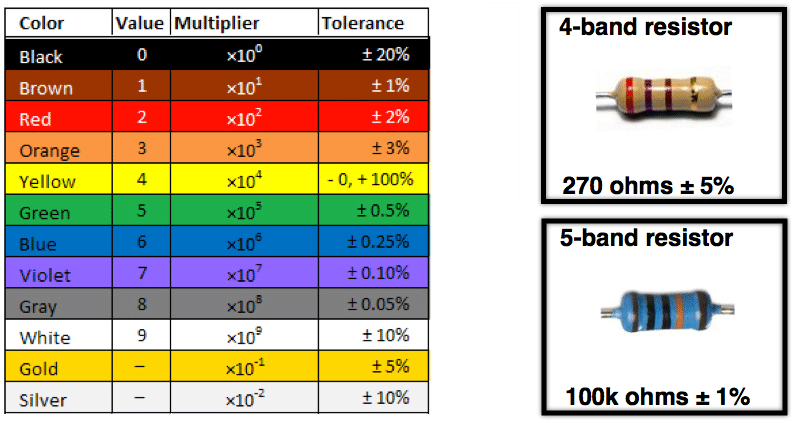
\includegraphics[width=0.8\textwidth]{Color-chart.png}
    \caption{Resistor color chart}
\end{figure}

\vspace{40pt}
\begin{minipage}{0.45\textwidth}
    \centering
    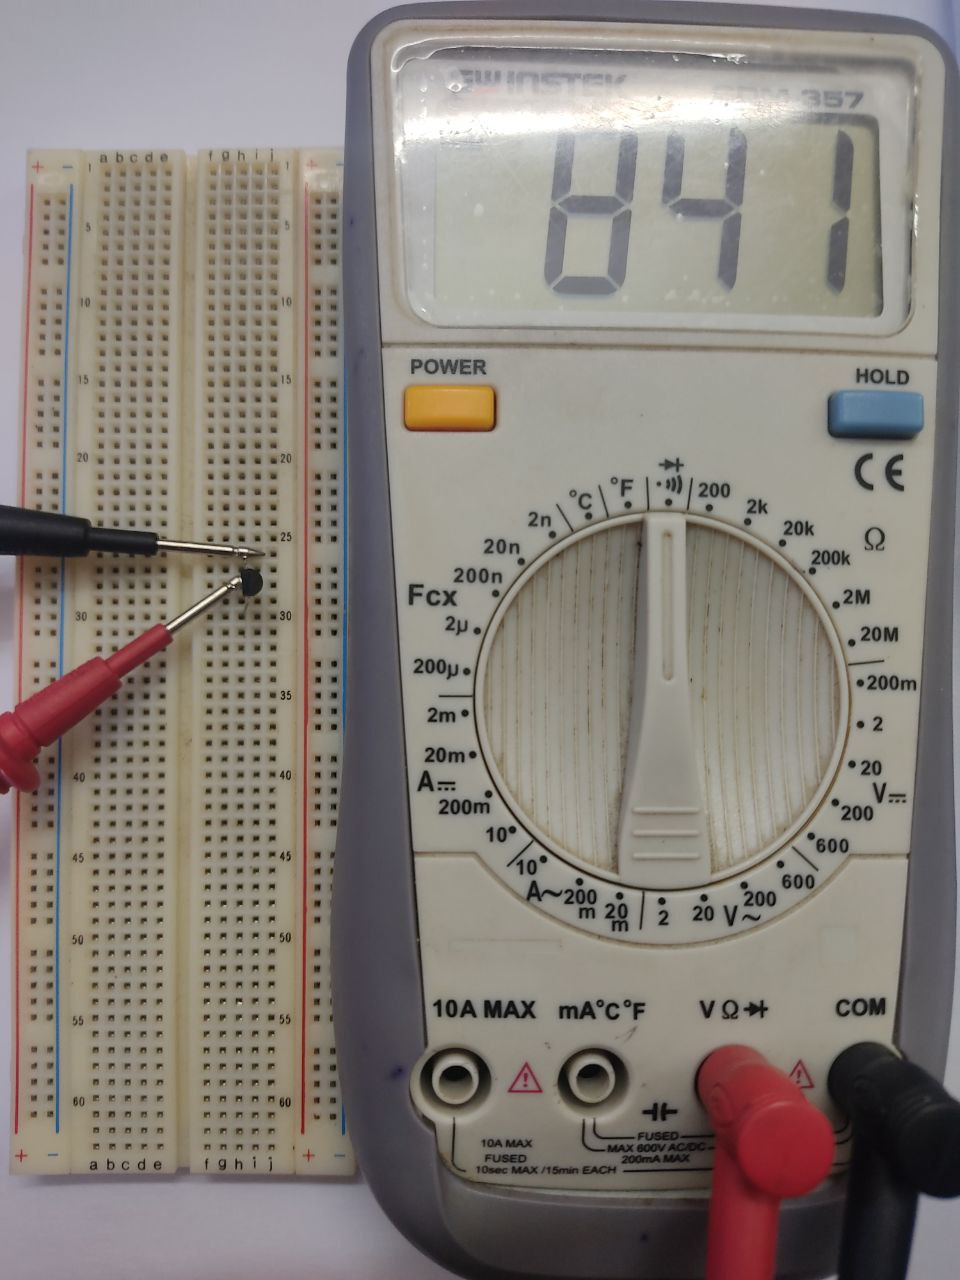
\includegraphics[width=0.8\textwidth]{npn.jpg}
    \captionof{figure}{n-p-n transistor}
\end{minipage}\hspace{30pt}
\begin{minipage}{0.45\textwidth}
    \centering
    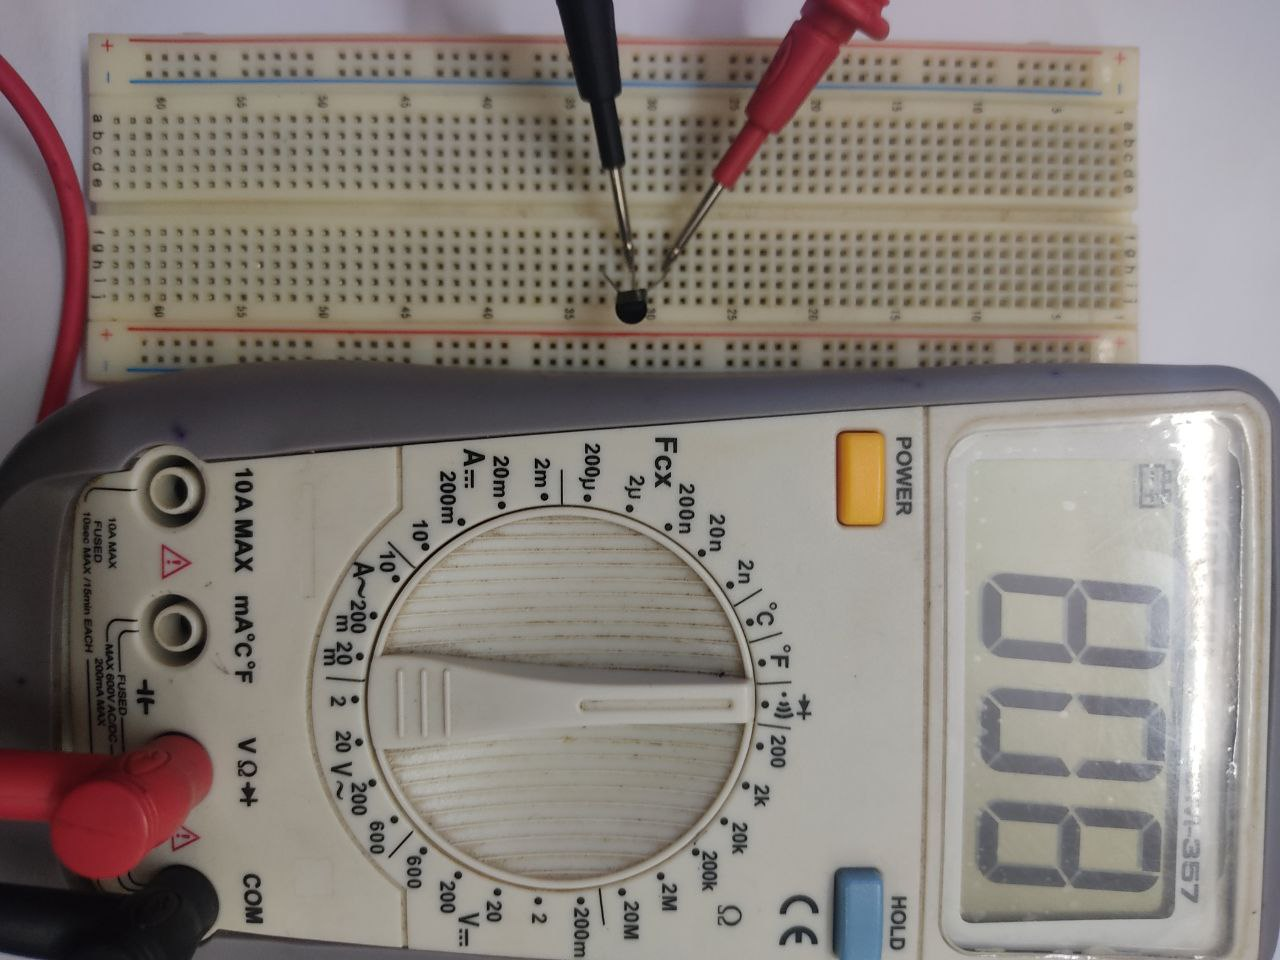
\includegraphics[angle=90, width=0.8\textwidth]{pnp.jpg}
    \captionof{figure}{p-n-p transistor}
\end{minipage}

\begin{minipage}{0.45\textwidth}
    \centering
    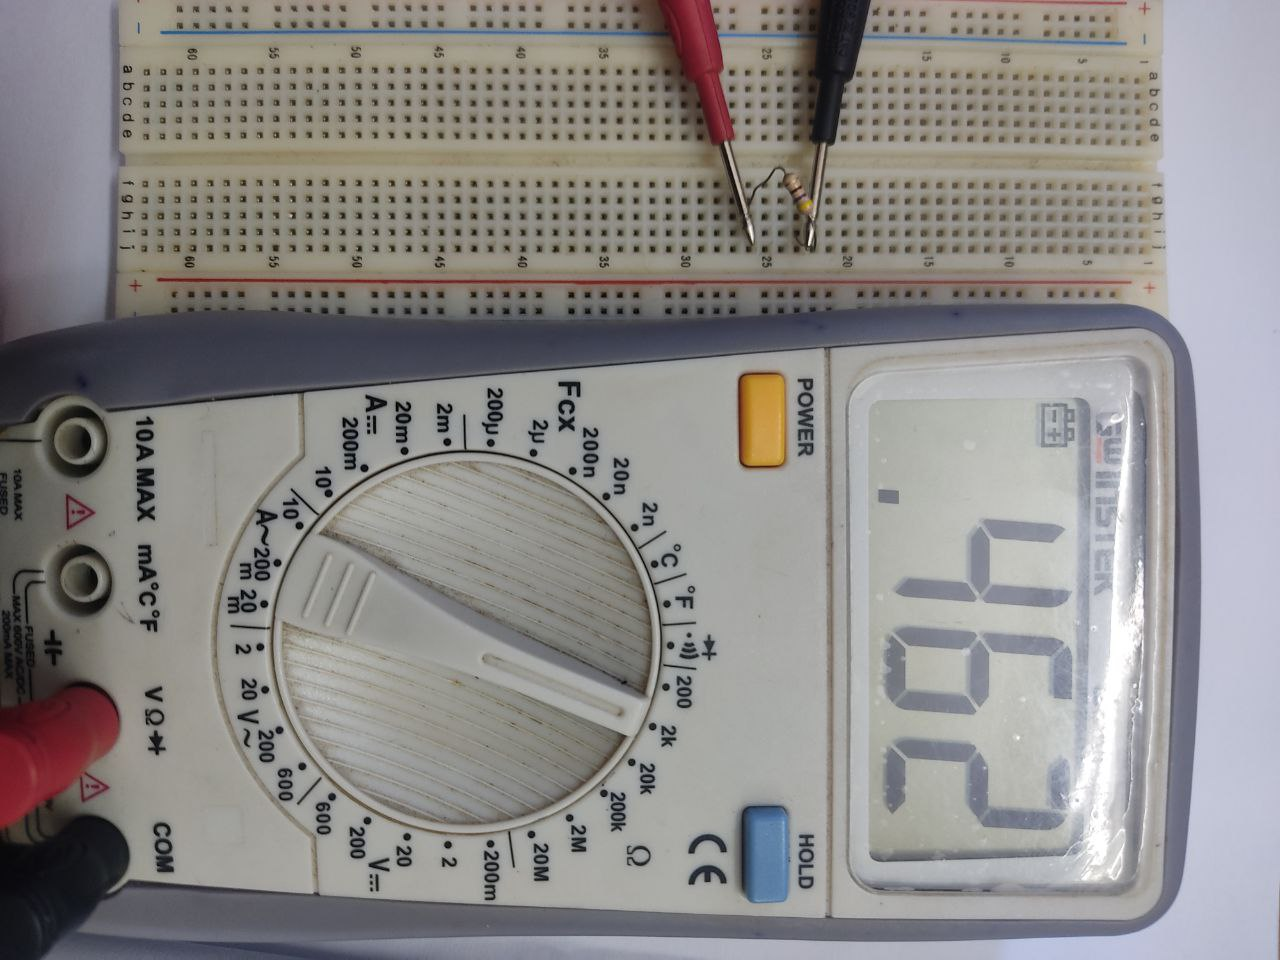
\includegraphics[angle=90, width=0.7\textwidth]{Res1.1.jpg}
    \captionof{figure}{462 $\Omega$ from multimeter}
\end{minipage}\hspace{30pt}
\begin{minipage}{0.45\textwidth}
    \centering
    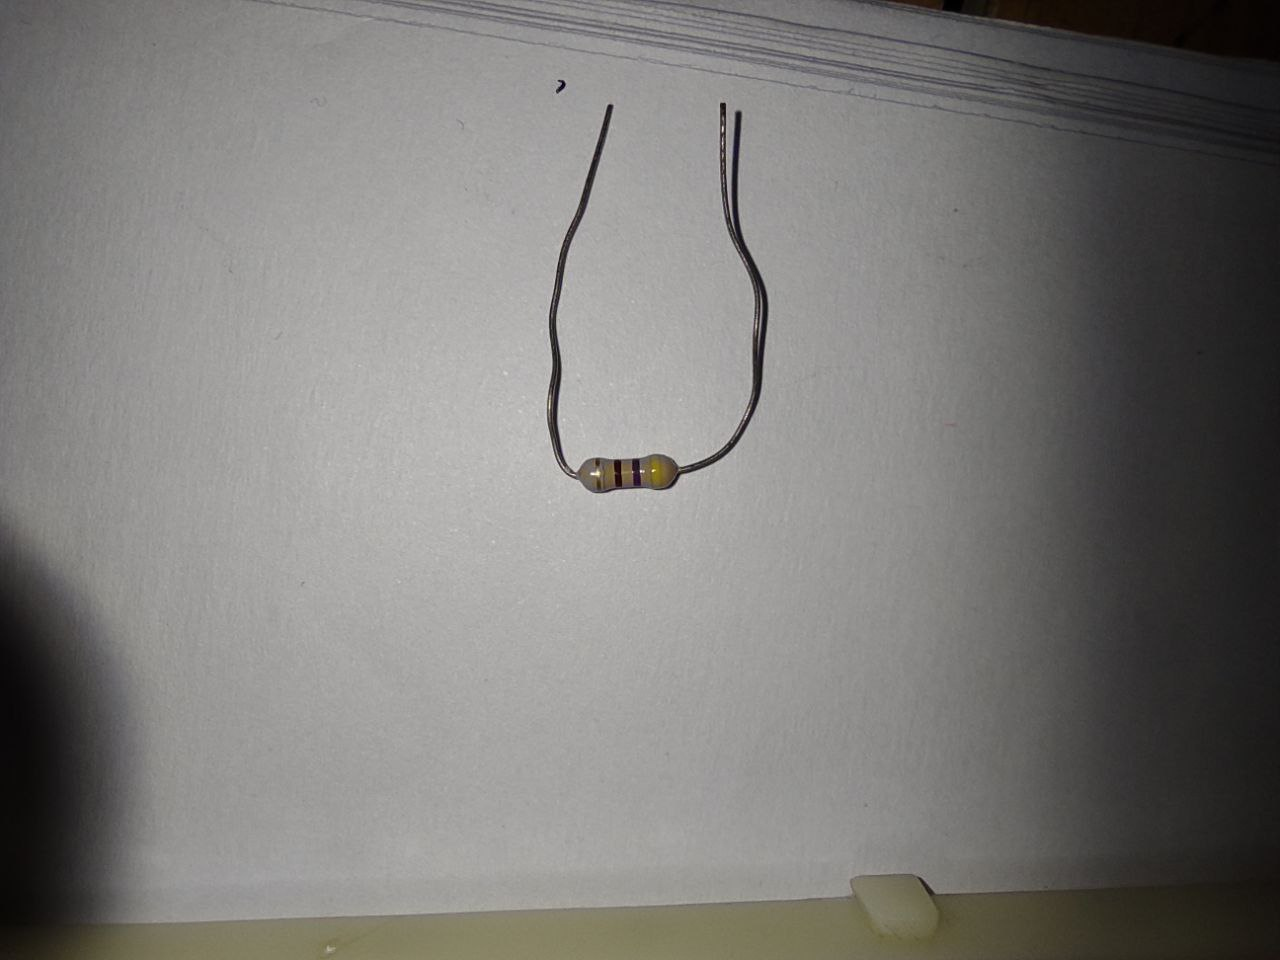
\includegraphics[angle=90, width=0.7\textwidth]{Res1.2.jpg}
    \captionof{figure}{460 $\Omega$ from color chart}
\end{minipage}

\begin{minipage}{0.45\textwidth}
    \centering
    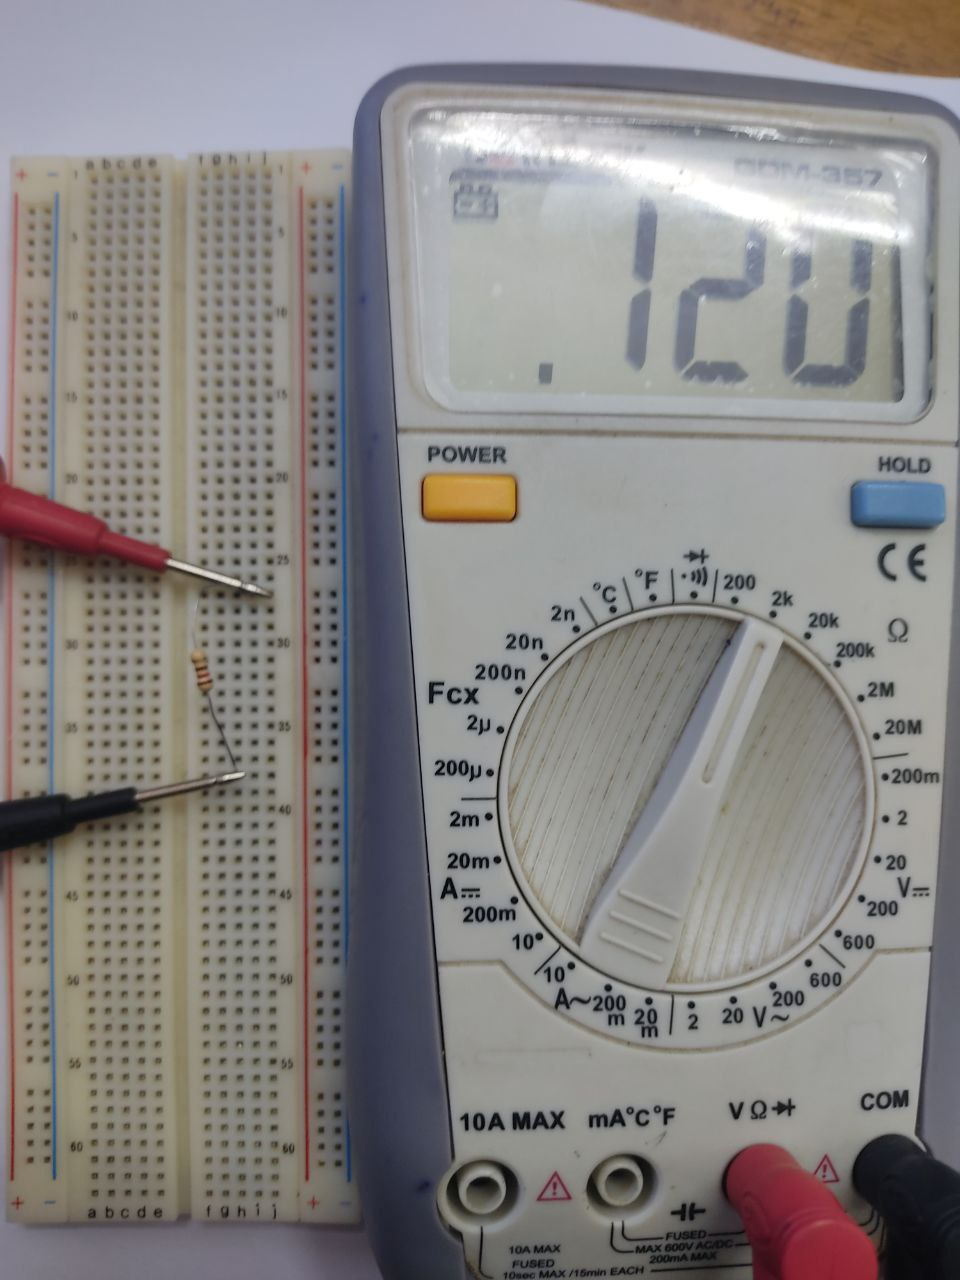
\includegraphics[width=0.7\textwidth]{Res2.1.jpg}
    \captionof{figure}{120 $\Omega$ from multimeter}
\end{minipage}\hspace{30pt}
\begin{minipage}{0.45\textwidth}
    \centering
    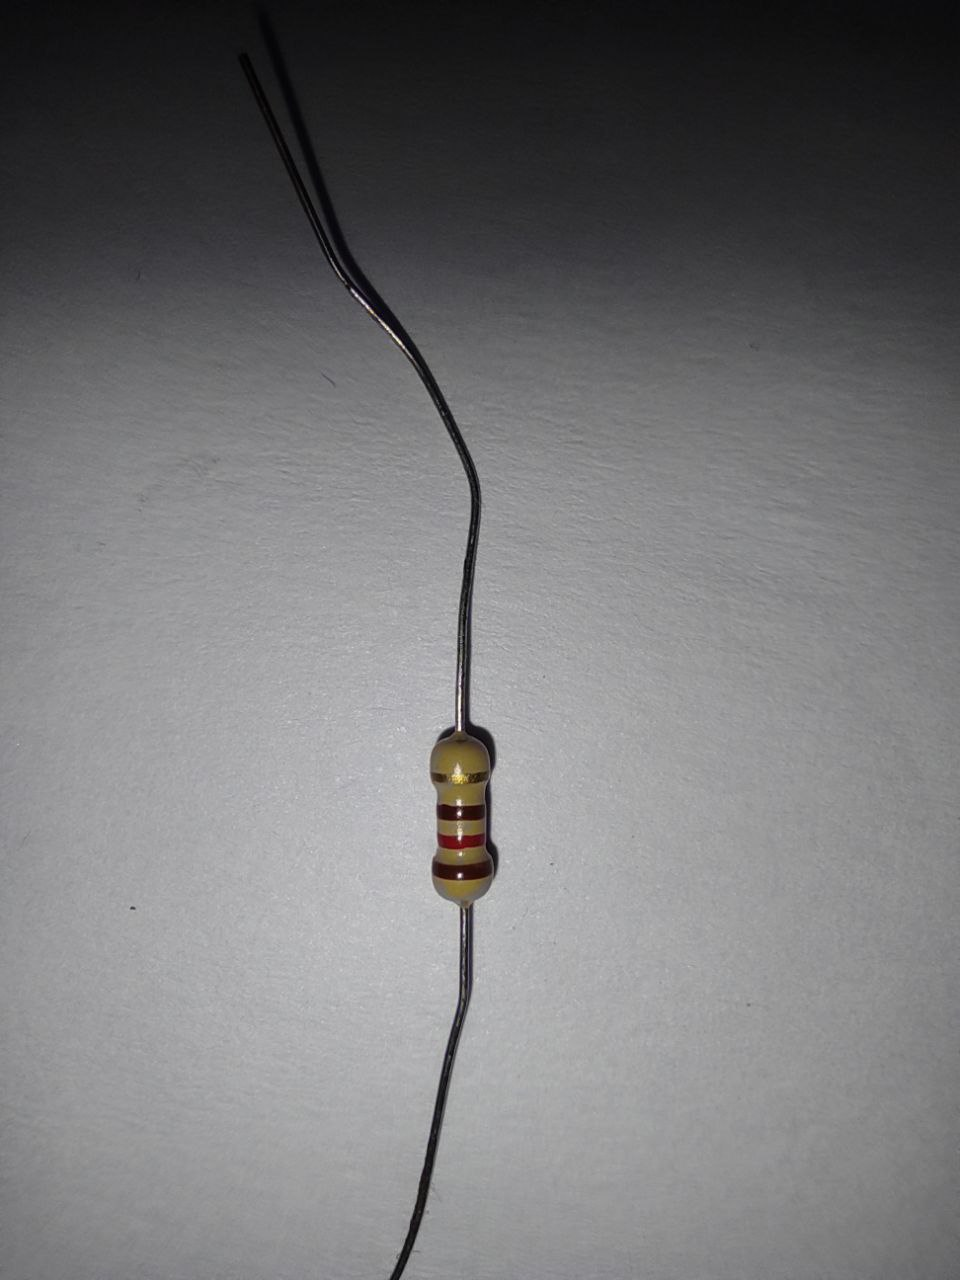
\includegraphics[angle=180, width=0.7\textwidth]{Res2.2.jpg}
    \captionof{figure}{120 $\Omega$ from color chart}
\end{minipage}

\begin{minipage}{0.45\textwidth}
    \centering
    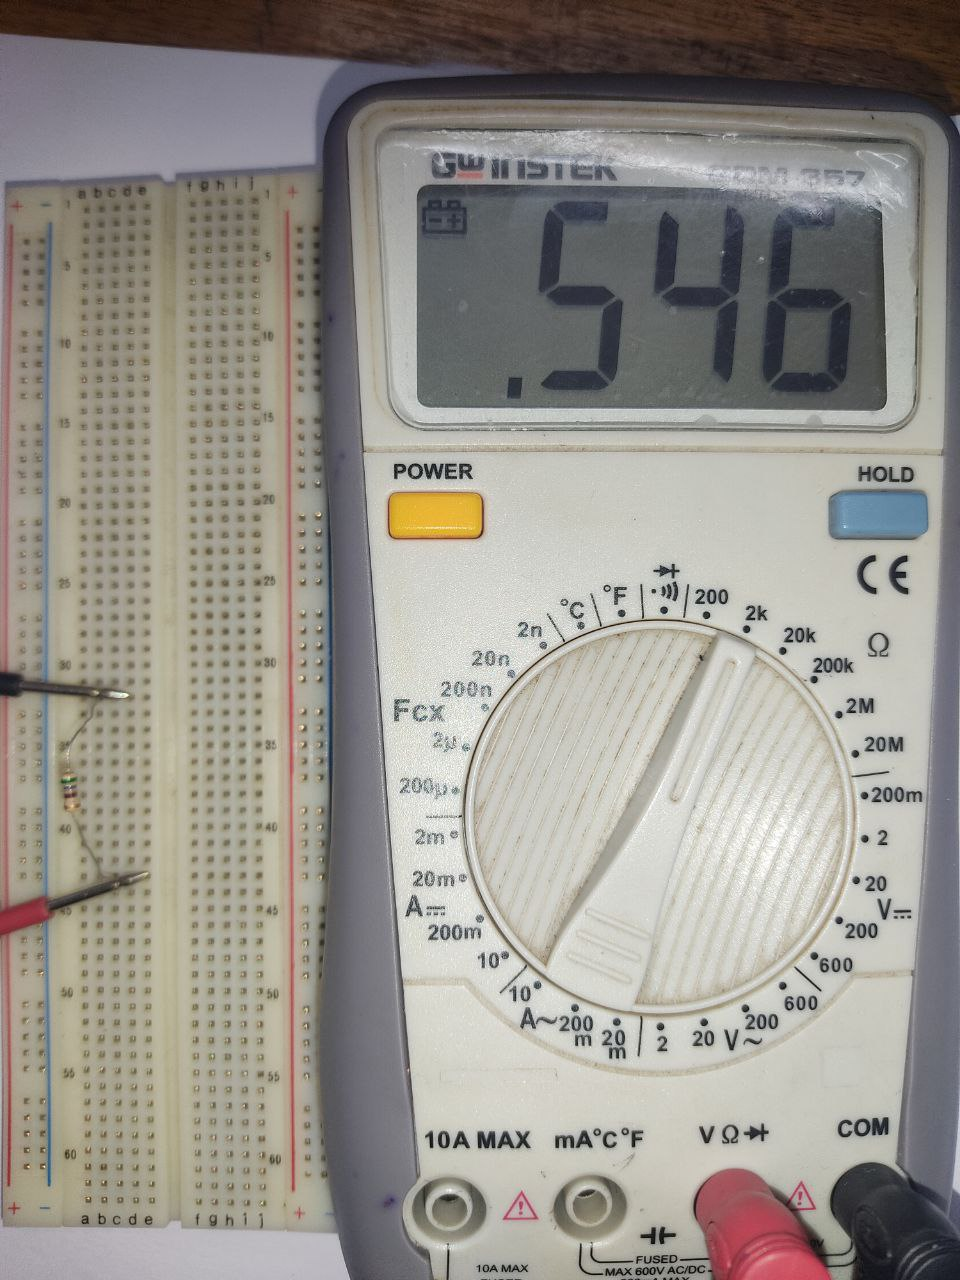
\includegraphics[width=0.7\textwidth]{Res3.1.jpg}
    \captionof{figure}{546 $\Omega$ from multimeter}
\end{minipage}\hspace{30pt}
\begin{minipage}{0.45\textwidth}
    \centering
    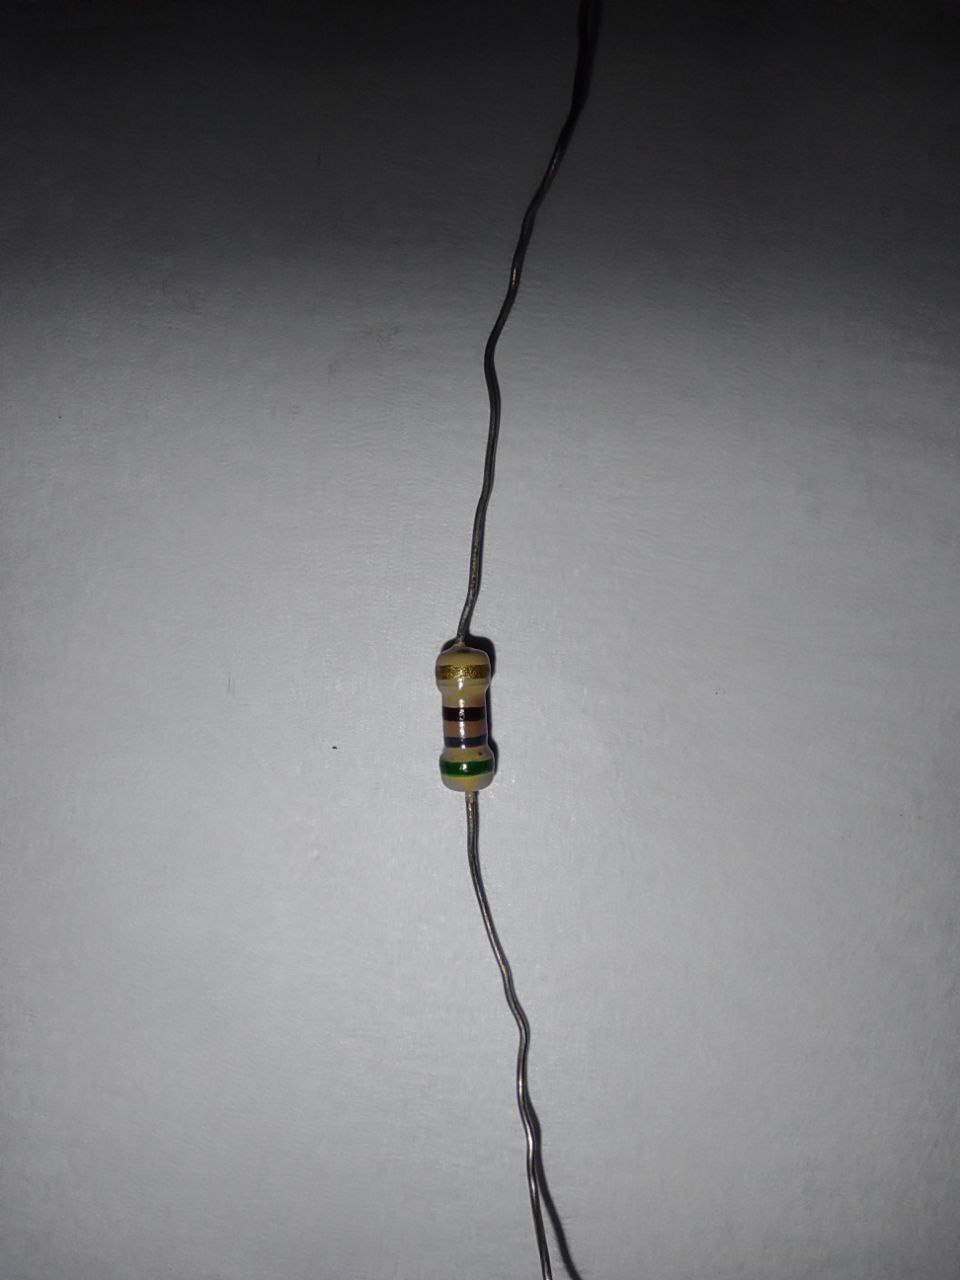
\includegraphics[angle=180, width=0.7\textwidth]{Res3.2.jpg}
    \captionof{figure}{560 $\Omega$ from color chart}
\end{minipage}

\newpage
\section{Procedure}
\subsection{Determining the value of a resistor}
\begin{enumerate}[(a)]
    \item A breadboard, multimeter, and three four colored resistors were taken in the first place. It was made sure that the multimeter was off and then the resistor was placed in the board.
    \item After turning the meter on, the resistance mode was activated. The meter has two probes -- the red probe and the black probe. Both were connected to two terminals of the resistor. As a result, a value was displayed in the multimeter.
    \item The first two colours of the resistor indicate the two leftmost digits of the resistance, whereas the 3rd one indicates the multiplier digit, and the 4th one declares the end of the calculation of resistor’s value.
    \item After the value was done measuring via multimeter, it was again measured using color chart. Figure-1 gives idea about the colour chart.
\end{enumerate}

\subsection{Finding out the nature of the transistor}
\begin{enumerate}[(a)]
    \item A 2N-3904 B331 transistor was taken in the first place. Then the multimeter's continuity mode was turned on by rotating the knob.
    \item The red probe was connected to the middle terminal of the transistor and the black probe was connected to one of the side terminals.
    \item If the transistor is n-p-n, then the multimeter will show a value. If it is p-n-p, then the multimeter will not show any value.
\end{enumerate}

\subsection{Identifying the terminals of the transistor}
\begin{enumerate}[(a)]
    \item The transistor has three terminals -- emitter, base, and collector. The base terminal is always in the middle and the side terminals are emitter and collector.
    \item A side terminal and the base terminal were connected to the multimeter. The same process was repeated for the other side terminal and the base terminal.
    \item The side terminal connection showing the larger value is emitter terminal, and the other one is collector terminal.
\end{enumerate}

\section{Discussion}
\begin{enumerate}
    \item The motive of the experiment was to measure the value of the resistor using color code with bare eyes and via multimeter, and also to check if the resistor is n-p-n or p-n-p.
    \item It was found that the value of the resistor was 462 $\Omega$ from multimeter and 460 $\Omega$ from color chart. The difference is negligible.
    \item Both n-p-n and p-n-p transistors were identified using multimeter.
    \item The measured values also matched with 2N-3904 n-p-n and other p-n-p transistor model. So, it can be said that the experiment was conducted properly.
\end{enumerate}

\end{document}
